\documentclass{article}
\usepackage{ctex}  % 自动支持中文
\usepackage{geometry}
\geometry{a4paper, margin=1in}

\usepackage{graphicx}  
\usepackage{booktabs}    
\usepackage{cite}

\bibliographystyle{plain}

\begin{document}

\title{示例文档}
\author{你的名字}
\date{\today}
\maketitle

\section{引言}
这是一个支持中文和 BibTeX 的 LaTeX 示例文档。 你可以引用文献,例如 \cite{zhao2024autonomous}。

\section{方法}
这里是方法部分。
各特征层的尺寸及通道数如表\ref{tab:feature_map_sizes}所示:

\begin{table}[hbt]
    \centering
    \caption{MobileNetV4-Conv-L特征层的尺寸和通道数} 
    \label{tab:feature_map_sizes}
    \begin{tabular*}{0.75\textwidth}{@{\extracolsep{\fill}}ccc}
    \toprule
      特征层 & 尺寸 & 通道数 \\
    \midrule
      \(\times2\)  & \(H/2 \times W/2\)   & 24 \\
      \(\times4\)  & \(H/4 \times W/4\)   & 48 \\
      \(\times8\)  & \(H/8 \times W/8\)   & 96 \\
      \(\times16\) & \(H/16 \times W/16\) & 192 \\
      \(\times32\) & \(H/32 \times W/32\) & 960 \\
    \bottomrule
    \end{tabular*}
  \end{table}

\section{结论}
这是结论部分。
网络框架如图\ref{fig:basenetwork}所示:
\begin{figure}[hbt]
    \centering
    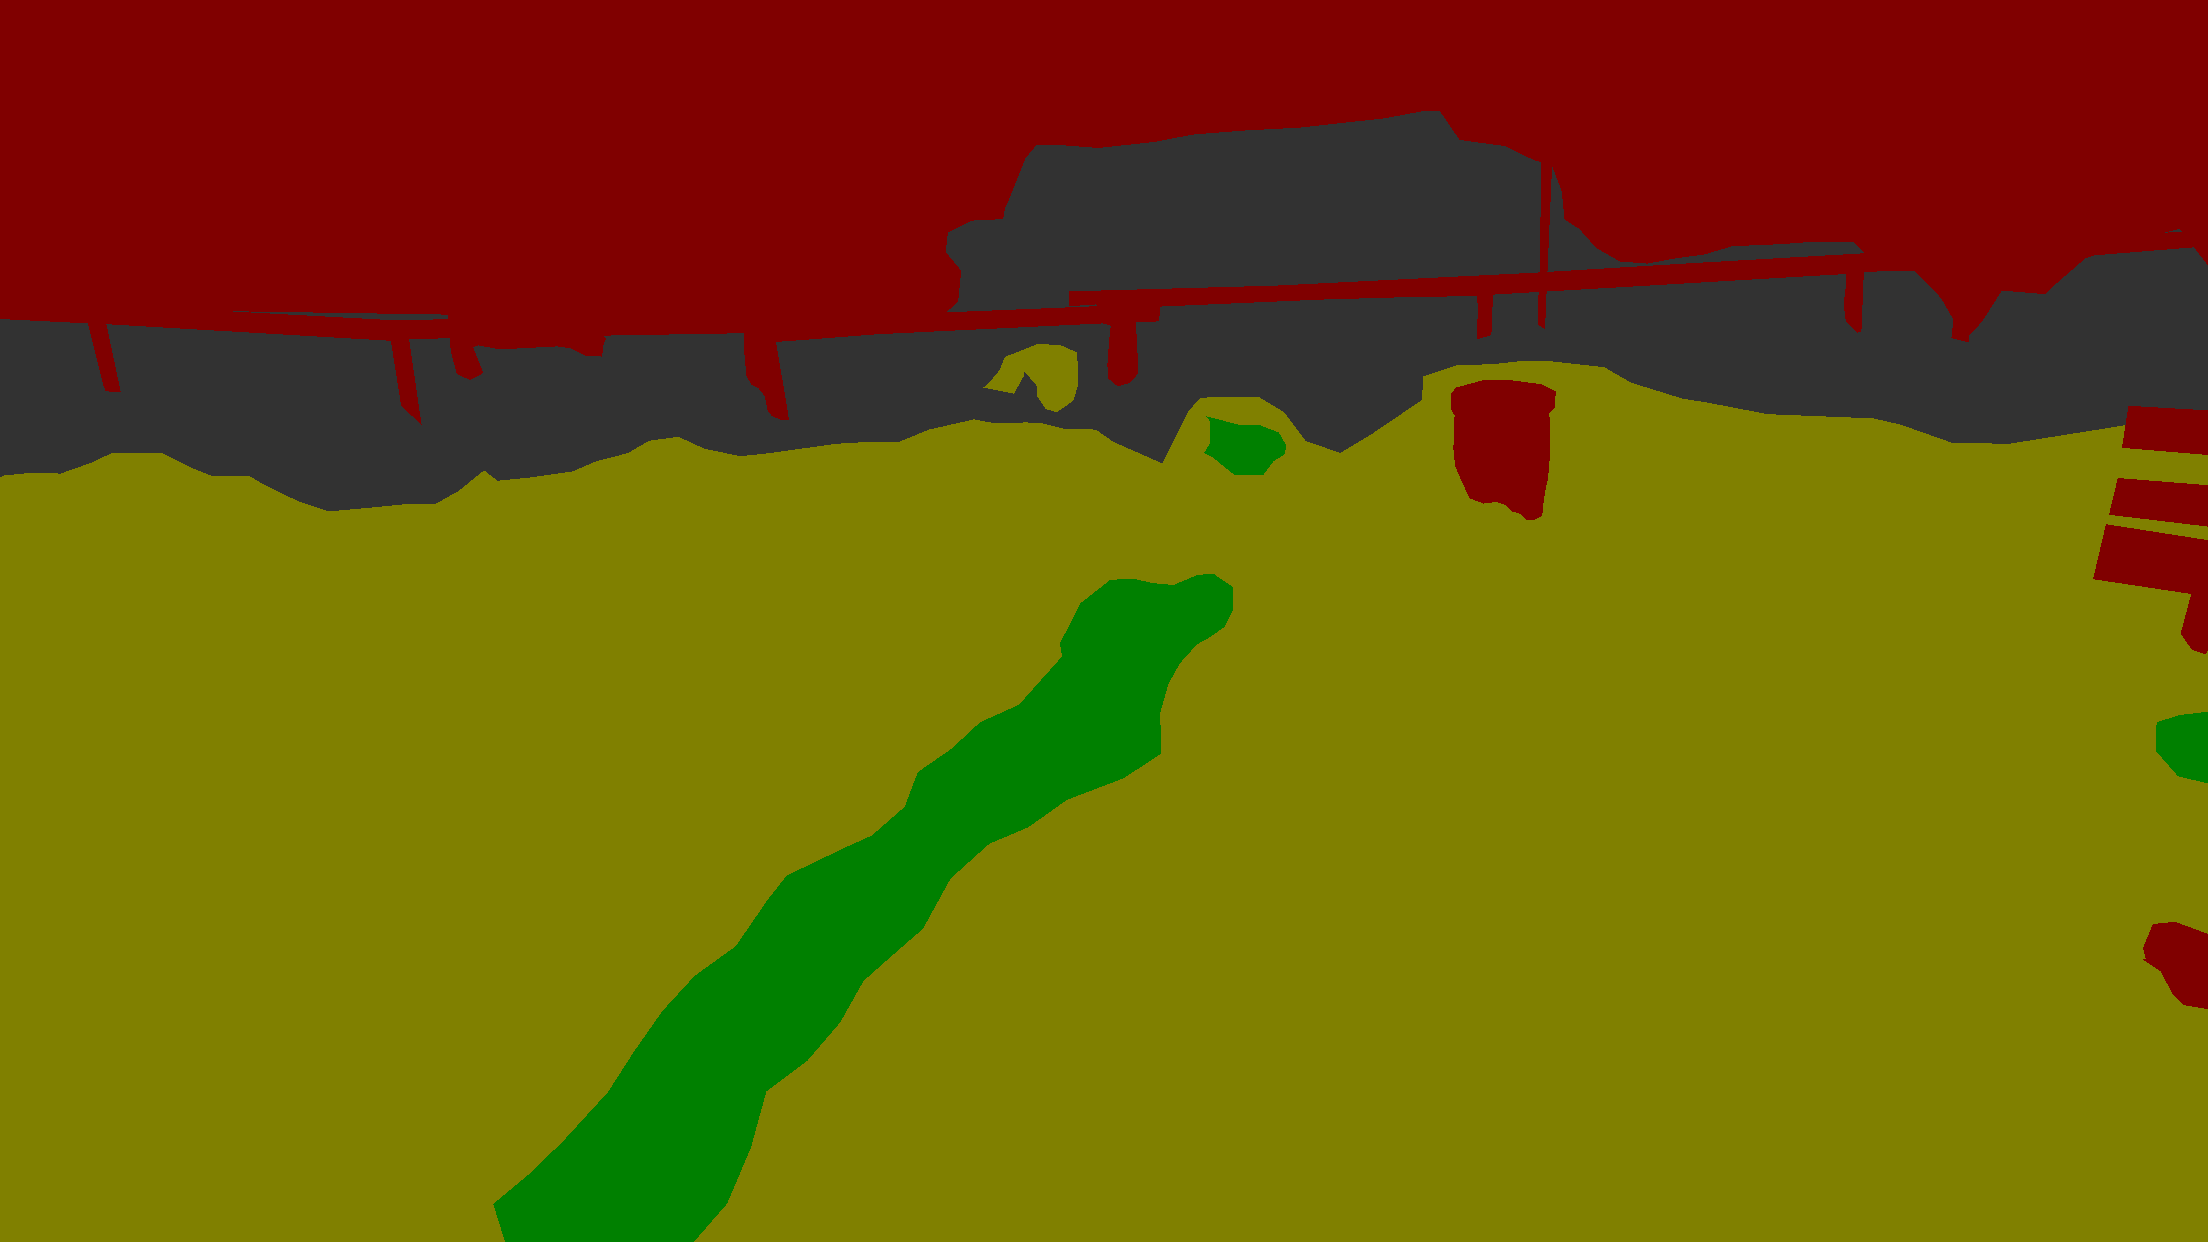
\includegraphics[width=0.5\textwidth]{figures/seg.png}
    % \caption[这里的文字将会显示在 listoffigure 中]{这里的文字将会显示在正文中}
    \caption{深度估计-语义分割联合网络框架}\label{fig:basenetwork}
   \end{figure}

\bibliography{main}

\end{document}
